% Chapter 4 - Description of Nek

\chapter{Application of Nek5000} % Main chapter title

\label{nek} % Change X to a consecutive number; for referencing this chapter elsewhere, use \ref{ChapterX}

\lhead{Chapter 4. \emph{application of Nek}} % Change X to a consecutive number; this is for the header on each page - perhaps a shortened title

%----------------------------------------------------------------------------------------
%	SECTION 1
%----------------------------------------------------------------------------------------


\colorbox{green}{ta med flyttdiagram for l;sningen}
\colorbox{green}{rydd opp i skjemaene! referer til en l;rerbok, beskriv vha numerisk flow phi\ldots }
\colorbox{green}{Hver tydelig paa hva man itererer over.}
\colorbox{green}{korte ned tekstene!}
There are many numerical solvers for turbulent flows available on the market.
From large commercial softwares such as Fluent which runs as a 
black-box solver, to full open-source codes such as Nek5000 and openFOAM. 
The solvers can vary in the numerical method; Finite volume, Finite Differences, 
Finite Element Method, Spectral Element Method etc. The particular algorithm 
for resolving the Pressure-Velocity coupling, for instance Fractional Step, Poisson pressure and 
Uzawa. The type of simulation available also varies from solver to solver, whether
they apply RANS, LES, DNS or something else. Although most solvers offer multiple of the settings
listed above it is important to be aware of their strengths and weaknesses before choosing which 
one to use. This section will be devoted to the handling of Nek5000 in particular, and can serve
as a brief introduction to the code.

\section{Nek5000 Basics}

Nek5000 is a turbulent flow solver developed mainly by Paul Fischer
and has through the past 20 years had several contributors. 
It is an open-source code applicable to many different types of flow 
and it has been put a lot of effort into the parallelization of the code, 
guaranteeing great speedup. All the parallelization is accessed through subroutines
and functions, enabling the user to make advanced functions without having to 
deal directly with the functions from the MPI library.
With SEM as the numerical method applied it is possible to obtain very accurate results.  

%nek5000 has its own mesh-generator for generating simpler geometries and it is also implemented the possibility to integrate CUBIT mesh 
%files. A common starting point for simulating turbulent flow is a geometry given by a CAD-file,
%without any functions to describe the boundaries.
%The possibility to make a mesh through a visual gui is provided through for instance ICEM.
%This mesh can then later be transformed to the inputfile required by Nek5000. 

Nek provides a basic tool for generation of mesh. For more complex geometries this tool cannot compare with more visualized-based softwares 
such as ICEM from ANSYS which exports mesh to several numerical solvers such as Fluent and Nastran.
It is therefore very useful to have an automatic way of converting a mesh created in ICEM to the format required by Nek5000. 
%In order for Nek to run optimally the elements should be as homogenous and as similar to the reference element as possible. 
%It is therefore of great interest to be able to propagate curved geometries into the neighbour-elements in order to have a smooth as 
%possible transition from a boundary with high curvature.

So far Nek5000 has supported three automatic routines for generating curved edges;
circles in 2-D geometries, spherical shell elements and a general 2nd degree interpolation.
Further manipulation of the element edges is left to the user to define manually
for each particular problem. One of the objectives of this thesis is to make Nek5000 more
user-friendly and create automatic routines to handle complex geometry. Before the work regarding
the mesh routines are further elaborated an overview of the file-structure will be presented.

\section{Editable files}
In order to work with Nek there are some practical information that needs to be clarified.
Nek is recompiled for every case and the user specify all the case specific 
information in the three files \verb|{.rea,.usr,SIZE,}|. The \verb|.usr| and \verb|SIZE| file are 
compiled with the standard Nek library using makenek which creates the executable file \verb|nek5000|,
while the \verb|.rea| file contains case-specific information read during initialization.
The user guide \cite{Nek} contains a tutorial which explains the necessary 
steps on how to get started with Nek. The next chapters will try to give some understanding on 
how the user is able to make the changes necessary for each case. Figure~\ref{fig:files} illustrates 
how the files work together. 
%
\begin{figure}[h]
	\centering
	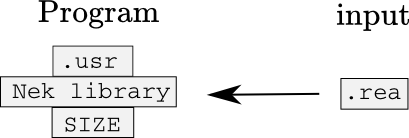
\includegraphics[width=0.5\textwidth]{Figures/filestructure2.png}
	\caption{Visualization of how the file structure in Nek5000 is built up.}
	\label{fig:files}
\end{figure}
%
%
\subsection{SIZE}
Since Nek is mostly based on Fortran77 all memory allocations are done statically and should be specified explicitly 
before runtime. Most of these variables are stated in \verb|SIZE|. The size of the working arrays 
necessary to perform the calculations are mostly defined by the upper limits of elements, 
processors, scalars and of course the polynomial degree
of the local Lagrange functions. These variables defines the sizes of almost all 
the arrays used in the program so it is important to define these variables as accurately 
as possible in order to optimize memory usage. The \verb|SIZE| file can be considered as the necessary base 
for Nek5000.
%\begingroup
%\fontsize{12pt}{14pt}
%\begin{lstlisting}[escapechar=|,frame=none]
%parameter (ldim=3)                                   ! dimension
%parameter (lx1=6,ly1=lx1,lz1=lx1,lelt=600,lelv=lelt) ! GLL-points,elements/processor
%parameter (lxd=9,lyd=lxd,lzd=lxd)                    ! Order of De-aliasing
%\end{lstlisting}
%\endgroup
\subsection{.rea}

%
\begin{table}
    \centering
    \begin{tabular}{c c l}[h]
       Lines & Section Name & Specifications \\ \hline
       $103$ & PARAMETERS & All problem-specific variables \\ 
       $K$ & PASSIVE SCALAR DATA & Convective and diffusive constants for scalars\\ 
       $K$ & LOGICAL SWITCHES & Boolean variables defining the solution method \\ 
       $E$ & MESH DATA & All nodes and elements are specified here\\
       $E$ & CURVED SIDE DATA & All the curved sides are specified here\\
       $E$ & FLUID BC& BCtype for all elements and their faces\\
       $E$ & THERMAL BC& Thermal BCtype for all elements and their faces\\
       $K$ & PRESOLVE/RESTART & Filename(s) of an initialized solution \\
       $K$ & INITIAL CONDITIONS & possibilities to specify IC further \\
       $K$ & OUTPUT FIELD & information that will be written to file \\
    \end{tabular}
    \caption{An overview of the different sections in .rea. $E$ is a predefined number depending on your problem
    which scales roughly as the number of elements, while $K\approx 1-25$ is user defined.}
    \label{tab:reafile}
\end{table}
%
In \verb|.rea| all the problem specific parameters are given. While the content in \verb|SIZE| 
is an absolute necessity to even compile the program the \verb|.rea| file contains variables 
that are not used until the initialization of the case. The structure of the file is given in table~\ref{tab:reafile}.
Of the 103 variables specified in the beginning of the file there are roughly 50 of them that are used. 
Note that apart from the mesh information the \verb|.rea| file restricts itself to single variables and boolean flags 
while the \verb|.usr| needs to be applied for more advanced implementations. 
\subsection{.usr}
This file contains a series of standard routines open for modification by the user. In addition the user is free to specify 
new routines if needed. A description of these routines are given in the Nek5000 User manual~\cite{Nek}. A list of those 
frequently used for this thesis are described below, 
%routines used for this thesis are stated in table~\ref{tab:userfile}.
%
%\begin{table}
    %\centering
    %\begin{tabular}{c l}
        %Name & Description \\ \hline
        %\verb|userbc| & boundary conditions \\
        %\verb|uservp| & variable properties\\
        %\verb|userchk|& general purpose routine for checking errors etc.\\
        %\verb|usrdat2|& redifining mesh properties \\
        %\verb|usrdat3|& similar to usrdat2 \\
    %\end{tabular}
    %\caption{routines in .usr applied for this thesis.}
    %\label{tab:userfile}
%\end{table}
%
\begin{itemize}
    \item \verb|userbc| - Define the boundary conditions on the inflow-boundary. 
    \item \verb|uservp| - Impose the eddy viscosity when applying LES. 
    \item \verb|userchk| - Read inflow-data, and specify the output.
    \item \verb|usrdat2| - Project the geometry onto a deformed general surface. The details of how this routine is used will be 
    specified further in chapter~\ref{implementation}. 
    \item \verb|usrdat3| - Defines the interpolation algorithm that is applied to the inflow-data. 
\end{itemize}
%
In addition to these routines all user-defined functions are specified in this file. The LES implementation in Nek is based
on several subroutines specified in addition to those stated above. A list of some of the variables and functions 
applied for the implementations in this thesis are stated in Appendix~\ref{AppendixB}.
The \verb|.usr| file can be considered as the surface of Nek5000, easily accessible for the user.

\section{Steps in the solver}
The most important building blocks in Nek5000 are the \verb|fluid| and \verb|heat| functions which solves the 
N-S and Passive scalar equations. For the sake of clarity, figure~\ref{fig:nek} shows how the different functions 
are called from the main routine.
%
\begin{figure}[h]
	\centering
	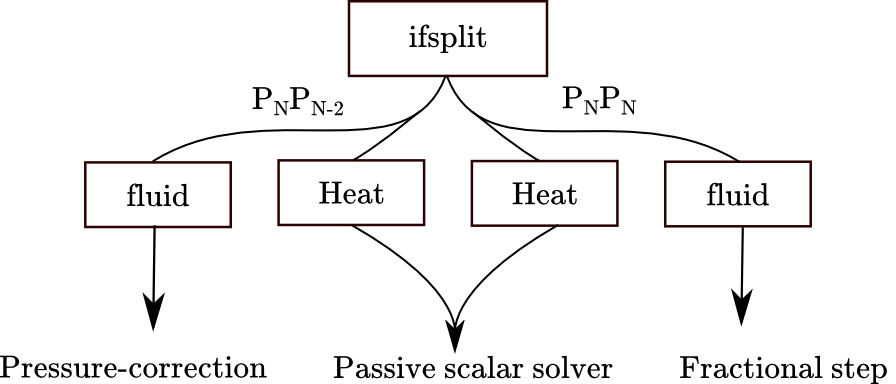
\includegraphics[width=0.8\textwidth]{Figures/Nek.png}
	\caption{Visualization of the steps in Nek5000.}
	\label{fig:files}
\end{figure}
%

To best understand the work flow of Nek the subroutine \verb|nek_advance| in \verb|drive1.f| should be examined.
This routine includes all the steps in one iteration of the solver. The routine is adapted so that it is functional
for a number of different problems and user defined settings. The most important boolean switches used in this routine are 
described in the list below 
%
\begin{itemize}
    \item ifsplit - whether the $\mathbb{P}_N-\mathbb{P}_N$ or the $\mathbb{P}_N-\mathbb{P}_{N-2}$ is to be used.
    \item iftrans - transient or steady flow.
    \item ifheat - solving for heat.
    \item ifnav - natural convection for the scalar fields (Boolean array)
    \item param(103) - activation of filtering.
\end{itemize}
%
further the routines of interests are \verb|fluid| and \verb|heat|, the solvers for N-S equations and passive scalars respectively.
Both subroutines are found in \verb|drive2.f|. The understanding of these solvers are best achieved by studying equation ~\ref{eq:NS} 
and~\ref{eq:PS}. For the settings chosen in this thesis a fractional step procedure as described in 
chapter~\ref{fracstep} is applied.

%\colorbox{yellow}{what are fluidp() and heatp( )? solve for pertubated field and then project onto div-free space ? }

\colorbox{yellow}{Talk about how the preconditioners work in Nek?}

%
%\section{Incompressible N-S solvers in Nek}
%Nek offer several implementations depending on the mathematical formulation wanted by the user.
%The most standard, and the algorithm applied in this thesis is the fractional step procedure 
%described in detail in chapter~\ref{description}.


%A Convection-Diffusion problem can be stated as 
%\begin{align}
    %M\frac{du}{dt} = Au-Cu+Mf
    %\label{eq:conv-diff}
%\end{align}
%% 
%Where $M$ and $A$ is the mass, and stiffness matrix, $f$ is the loading function and $C$ is 
%the matrix corresponding to the convective term. The non-linearity is represented in the 
%convective term since $C$ is dependent of $u$.
%The time-derivative is discretized by a Backward difference (BDFk) scheme using solutions 
%from the $k$ previous steps to extrapolate the current value. In order to gain stability 
%an implicit scheme is chosen and the resulting eguation is given as 
%%
%OIFS ???
%---------- CHECK MAKEF IN NAVIER1.F ----------------- 
%\begin{align}
    %\sum_{j=0}^{k}\frac{b_j}{\Delta t}Mu^{n-j+1} = Au^{n+1}-Cu^{n+1}+Mf^{n+1}
    %\label{eq:conv-diff2}
%\end{align}
%% 
%By extrapolating the convective term from the $k$ previously calculated steps the equation 
%simplifies to 
%%
%\begin{align}
   %\frac{b_0}{\Delta t}Mu^{n+1} \sum_{j=1}^{k}\frac{b_j}{\Delta t}Mu^{n-j+1} 
   %= Au^{n+1}-\sum_{j=1}^{k}a_jCu^{n-j+1}+Mf^{n+1}
    %\label{eq:conv-diff3}
%\end{align}
%% 
%and finally by moving all the explicit terms to the rhs the equation left to solve is given as 
%%
%\begin{align}
   %(\frac{b_0}{\Delta t}M-A)u^{n+1} 
   %= -\sum_{j=1}^{k}(\frac{b_j}{\Delta t}M-a_jC)u^{n-j+1}+Mf^{n+1}
    %\label{eq:conv-diff4}
%\end{align}
%% 
%Notice from Section~\ref{theory} that this is equivalent to the matrix formulation of 
%the Helmholtz equation.



\section{Nek5000 for complex geometries}
For complex curved geometries such as bent cylinders, spheres, ellipsoidals etc.
the user has to be able to express these surfaces analytically and write a routine
in \verb|usrdat2| that projects the points of interest onto the surface.
Even for a simple shape such as a sphere some implementation has to be done and it 
demands that the user has knowledge to Fortran77 and the structure of Nek5000.

The necessary implementation consists of two steps 
%
\begin{enumerate}
    \item determine the faces that belongs to the deformed surface
    \item project the predefined GLL-points onto the deformed surface
\end{enumerate}
%
This can be done without too much work for shapes with a known analytical 
expression such as a cylinder or a sphere, but for some general CAD geometry 
it is no way to perform this projection routine. 

Many turbulent solvers does not support curved elements simply because the 
complex geometries are resolved with a sufficiently high resolution and it 
is of no interest to approximate them any better. However for a spectral element
solver it is necessary to address this problem since the initial grid is a lot coarser
compared to equivalent settings in other solvers.

\colorbox{green}{Comment on the MOAB possibility??}


